\documentclass[10pt,a4paper,oneside,fleqn]{article}
\usepackage{geometry}
\geometry{a4paper,left=20mm,right=20mm,top=1cm,bottom=2cm}
\usepackage[utf8]{inputenc}
%\usepackage{ngerman}
\usepackage{amsmath}                % brauche ich um dir Formel zu umrahmen.
\usepackage{amsfonts}                % brauche ich für die Mengensymbole
\usepackage{graphicx}
\setlength{\parindent}{0px}
\setlength{\mathindent}{10mm}
\usepackage{bbold}                    %brauche ich für die doppel Zahlen Darstellung (Einheitsmatrix z.B)



\usepackage{color}
\usepackage{titlesec} %sudo apt-get install texlive-latex-extra

\definecolor{darkblue}{rgb}{0.1,0.1,0.55}
\definecolor{verydarkblue}{rgb}{0.1,0.1,0.35}
\definecolor{darkred}{rgb}{0.55,0.2,0.2}

%hyperref Link color
\usepackage[colorlinks=true,
        linkcolor=darkblue,
        citecolor=darkblue,
        filecolor=darkblue,
        pagecolor=darkblue,
        urlcolor=darkblue,
        bookmarks=true,
        bookmarksopen=true,
        bookmarksopenlevel=3,
        plainpages=false,
        pdfpagelabels=true]{hyperref}

\titleformat{\chapter}[display]{\color{darkred}\normalfont\huge\bfseries}{\chaptertitlename\
\thechapter}{20pt}{\Huge}

\titleformat{\section}{\color{darkblue}\normalfont\Large\bfseries}{\thesection}{1em}{}
\titleformat{\subsection}{\color{verydarkblue}\normalfont\large\bfseries}{\thesubsection}{1em}{}

% Notiz Box
\usepackage{fancybox}
\newcommand{\notiz}[1]{\vspace{5mm}\ovalbox{\begin{minipage}{1\textwidth}#1\end{minipage}}\vspace{5mm}}

\usepackage{cancel}
\setcounter{secnumdepth}{3}
\setcounter{tocdepth}{3}





%-------------------------------------------------------------------------------
%Diff-Makro:
%Das Diff-Makro stellt einen Differentialoperator da.
%
%Benutzung:
% \diff  ->  d
% \diff f  ->  df
% \diff^2 f  ->  d^2 f
% \diff_x  ->  d/dx
% \diff^2_x  ->  d^2/dx^2
% \diff f_x  ->  df/dx
% \diff^2 f_x  ->  d^2f/dx^2
% \diff^2{f(x^5)}_x  ->  d^2(f(x^5))/dx^2
%
%Ersetzt man \diff durch \pdiff, so wird der partieller
%Differentialoperator dargestellt.
%
\makeatletter
\def\diff@n^#1{\@ifnextchar{_}{\diff@n@d^#1}{\diff@n@fun^#1}}
\def\diff@n@d^#1_#2{\frac{\textrm{d}^#1}{\textrm{d}#2^#1}}
\def\diff@n@fun^#1#2{\@ifnextchar{_}{\diff@n@fun@d^#1#2}{\textrm{d}^#1#2}}
\def\diff@n@fun@d^#1#2_#3{\frac{\textrm{d}^#1 #2}{\textrm{d}#3^#1}}
\def\diff@one@d_#1{\frac{\textrm{d}}{\textrm{d}#1}}
\def\diff@one@fun#1{\@ifnextchar{_}{\diff@one@fun@d #1}{\textrm{d}#1}}
\def\diff@one@fun@d#1_#2{\frac{\textrm{d}#1}{\textrm{d}#2}}
\newcommand*{\diff}{\@ifnextchar{^}{\diff@n}
  {\@ifnextchar{_}{\diff@one@d}{\diff@one@fun}}}
%
%Partieller Diff-Operator.
\def\pdiff@n^#1{\@ifnextchar{_}{\pdiff@n@d^#1}{\pdiff@n@fun^#1}}
\def\pdiff@n@d^#1_#2{\frac{\partial^#1}{\partial#2^#1}}
\def\pdiff@n@fun^#1#2{\@ifnextchar{_}{\pdiff@n@fun@d^#1#2}{\partial^#1#2}}
\def\pdiff@n@fun@d^#1#2_#3{\frac{\partial^#1 #2}{\partial#3^#1}}
\def\pdiff@one@d_#1{\frac{\partial}{\partial #1}}
\def\pdiff@one@fun#1{\@ifnextchar{_}{\pdiff@one@fun@d #1}{\partial#1}}
\def\pdiff@one@fun@d#1_#2{\frac{\partial#1}{\partial#2}}
\newcommand*{\pdiff}{\@ifnextchar{^}{\pdiff@n}
  {\@ifnextchar{_}{\pdiff@one@d}{\pdiff@one@fun}}}
\makeatother
%
%Das gleich nur mit etwas andere Syntax. Die Potenz der Differentiation wird erst
%zum Schluss angegeben. Somit lautet die Syntax:
%
% \diff_x^2  ->  d^2/dx^2
% \diff f_x^2  ->  d^2f/dx^2
% \diff{f(x^5)}_x^2  ->  d^2(f(x^5))/dx^2
% Ansonsten wie Oben.
%
%Ersetzt man \diff durch \pdiff, so wird der partieller
%Differentialoperator dargestellt.
%
%\makeatletter
%\def\diff@#1{\@ifnextchar{_}{\diff@fun#1}{\textrm{d} #1}}
%\def\diff@one_#1{\@ifnextchar{^}{\diff@n{#1}}%
%  {\frac{\textrm d}{\textrm{d} #1}}}
%\def\diff@fun#1_#2{\@ifnextchar{^}{\diff@fun@n#1_#2}%
%  {\frac{\textrm d #1}{\textrm{d} #2}}}
%\def\diff@n#1^#2{\frac{\textrm d^#2}{\textrm{d}#1^#2}}
%\def\diff@fun@n#1_#2^#3{\frac{\textrm d^#3 #1}%
%  {\textrm{d}#2^#3}}
%\def\diff{\@ifnextchar{_}{\diff@one}{\diff@}}
%\newcommand*{\diff}{\@ifnextchar{_}{\diff@one}{\diff@}}
%
%Partieller Diff-Operator.
%\def\pdiff@#1{\@ifnextchar{_}{\pdiff@fun#1}{\partial #1}}
%\def\pdiff@one_#1{\@ifnextchar{^}{\pdiff@n{#1}}%
%  {\frac{\partial}{\partial #1}}}
%\def\pdiff@fun#1_#2{\@ifnextchar{^}{\pdiff@fun@n#1_#2}%
%  {\frac{\partial #1}{\partial #2}}}
%\def\pdiff@n#1^#2{\frac{\partial^#2}{\partial #1^#2}}
%\def\pdiff@fun@n#1_#2^#3{\frac{\partial^#3 #1}%
%  {\partial #2^#3}}
%\newcommand*{\pdiff}{\@ifnextchar{_}{\pdiff@one}{\pdiff@}}
%\makeatother

%-------------------------------------------------------------------------------
%%Nützliche Makros um in der Quantenmechanik Bras, Kets und das Skalarprodukt
%%zwischen den beiden darzustellen.
%%Benutzung:
%% \bra{x}  ->    < x |
%% \ket{x}  ->    | x >
%% \braket{x}{y} ->   < x | y >

\newcommand\bra[1]{\left\langle #1 \right|}
\newcommand\ket[1]{\left| #1 \right\rangle}
\newcommand\braket[2]{%
  \left\langle #1\vphantom{#2} \right.%
  \left|\vphantom{#1#2}\right.%
  \left. \vphantom{#1}#2 \right\rangle}%

%-------------------------------------------------------------------------------
%%Aus dem Buch:
%%Titel:  Latex in Naturwissenschaften und Mathematik
%%Autor:  Herbert Voß
%%Verlag: Franzis Verlag, 2006
%%ISBN:   3772374190, 9783772374197
%%
%%Hier werden drei Makros definiert:\mathllap, \mathclap und \mathrlap, welche
%%analog zu den aus Latex bekannten \rlap und \llap arbeiten, d.h. selbst
%%keinerlei horizontalen Platz benötigen, aber dennoch zentriert zum aktuellen
%%Punkt erscheinen.

\newcommand*\mathllap{\mathstrut\mathpalette\mathllapinternal}
\newcommand*\mathllapinternal[2]{\llap{$\mathsurround=0pt#1{#2}$}}
\newcommand*\clap[1]{\hbox to 0pt{\hss#1\hss}}
\newcommand*\mathclap{\mathpalette\mathclapinternal}
\newcommand*\mathclapinternal[2]{\clap{$\mathsurround=0pt#1{#2}$}}
\newcommand*\mathrlap{\mathpalette\mathrlapinternal}
\newcommand*\mathrlapinternal[2]{\rlap{$\mathsurround=0pt#1{#2}$}}

%%Das Gleiche nur mit \def statt \newcommand.
%\def\mathllap{\mathpalette\mathllapinternal}
%\def\mathllapinternal#1#2{%
%  \llap{$\mathsurround=0pt#1{#2}$}% $
%}
%\def\clap#1{\hbox to 0pt{\hss#1\hss}}
%\def\mathclap{\mathpalette\mathclapinternal}
%\def\mathclapinternal#1#2{%
%  \clap{$\mathsurround=0pt#1{#2}$}%
%}
%\def\mathrlap{\mathpalette\mathrlapinternal}
%\def\mathrlapinternal#1#2{%
%  \rlap{$\mathsurround=0pt#1{#2}$}% $
%}

%-------------------------------------------------------------------------------
%%Hier werden zwei neue Makros definiert \overbr und \underbr welche analog zu
%%\overbrace und \underbrace funktionieren jedoch die Gleichung nicht
%%'zerreißen'. Dies wird ermöglicht durch das \mathclap Makro.

\def\overbr#1^#2{\overbrace{#1}^{\mathclap{#2}}}
\def\underbr#1_#2{\underbrace{#1}_{\mathclap{#2}}}

\usepackage{amsmath}                % brauche ich um dir Formel zu umrahmen.

\begin{document}
\section*{Wasserstoffatom}

Das Wasserstoffatom ist das einfachste cheminsche Element. Es besteht aus einem Proton und einem Elektron. Isotope enthalten zusätzlich Neutronen im Kern. Aus quanenmechanischer Sicht ist das H-Atom einzige Element das exakt beschrieben werden kann. 

Der Hamilton-Operator allgemein lautet:

\begin{equation}
  \label{eq:1}
  H = -\frac{\hbar^2}{2m_p}\nabla^2_p - \frac{\hbar^2}{2m_{e}}\nabla^2_e - \frac{e^2}{|\vec r_p-\vec r_e|}
\end{equation}

Wir wollen den Hamilton in Schwerpunktskoordinaten ausdrücken.

\begin{equation}
  \label{eq:2}
  \vec R = \frac{m_e\vec r_e + m_p\vec r_p}{m_e+m_p} \qquad \vec r = \vec r_e-\vec r_p
\end{equation}

Für den Gradienten im Schwerpunkssystem gilt ebenfalls die Impulserhaltung:

\begin{equation}
  \label{eq:3}
  \frac{1}{2m_e}\nabla_e^2 + \frac{1}{2m_p}\nabla_p^2 = \frac{1}{2M}\nabla_R^2 + \frac{1}{2\mu}\nabla_r^2
\end{equation}

Mit

\begin{equation}
  \label{eq:5}
  M = m_p+m_e\qquad \mu = \frac{m_em_p}{m_e+m_p}
\end{equation}

Der Hamilton-Operator \eqref{eq:1} sieht nach Ersetzung wie folgt aus:

\begin{equation}
  \label{eq:4}
  H = -\frac{\hbar^2}{2M}\nabla^2_R - \frac{\hbar^2}{2\mu}\nabla^2_r - \frac{e^2}{r}
\end{equation}

Hamilton-Operator in die Schrödinger-Gleichung eingesetzt:

\begin{align}
  \label{eq:6}
  H\Psi(\vec R,\vec r) &= E\Psi(\vec R,\vec r) \\
\left[-\frac{\hbar^2}{2M}\nabla^2_R - \frac{\hbar^2}{2\mu}\nabla^2_r - \frac{e^2}{r}\right]\Psi(\vec R,\vec r) &= E\Psi(\vec R,\vec r) \\
\end{align}
Es ist günstig ein Producktansatz für die beiden Relativkoordinaten \(\vec R,\vec r\) anzusetzen:

\begin{equation}
  \label{eq:7}
  \Psi(\vec R,\vec r) = \Phi(\vec R) \cdot \psi(\vec r)
\end{equation}

Eingesetzt in \eqref{eq:6} erhalten wir die Relativkoordinaten \(\vec R,\vec r\) separiert in zwei Summanten:

\begin{equation}
  \label{eq:8}
  \left[-\frac{\hbar^2}{2M}\frac{1}{\Phi(\vec R)}\nabla_R^2\Phi(\vec R)  \right]+\left[-\frac{\hbar^2}{2\mu}\frac{1}{\psi(\vec r)}\nabla_r^2\psi(\vec r) - \frac{e^2}{r} \right] = E_R+E_r
\end{equation}

Da erste Klammer nur von \(\vec R\) und die zweite Klammer von \(\vec r\) abhängt und beide  \(\vec R,\vec r\) voneinander unabhängige Vektoren sind, müssen beide Klammern unabhängig voneinander einer Konstanten entsprechen. Somit bekommen wir zwei Gleichungen:

\begin{align}
 -\frac{\hbar^2}{2M}\frac{1}{\Phi(\vec R)}\nabla_R^2\Phi(\vec R)  &= E_R\Phi(\vec R) \label{eq:9} \\
\left[-\frac{\hbar^2}{2\mu}\nabla_r^2 - \frac{e^2}{r} \right]\psi(\vec r) &= E_r\psi(\vec r) \label{eq:10}
\end{align}

Aus der Gleichung \eqref{eq:9} sieht man dass der Schwerpunkt sich wie ein freies Teilchen verhält mit der Lösung der Ebenen Wellen:

\begin{equation}
  \label{eq:11}
  \Phi(\vec R) = \left( \frac{1}{\sqrt{2\pi}}\right)^3 e^{i\vec k\cdot\vec R}
\end{equation}

Mit der Zugehörigen Energie

\begin{equation}
  \label{eq:12}
  E_R = \frac{\hbar^2k^2}{2M}
\end{equation}

Da die Gleichung \eqref{eq:10} ein fiktives Teilchen mit der Masse \(\mu\) beschreibt, das sich in einem Zentralen Potential \(-\frac{e^2}{r}\) bewegt wird in den meisten Fällen nur diese Gleichung bei Zentralpotentialproblemen wie dem H-Atom betrachtet.

\subsection*{Lösung der Schröginger-Gleichung für ein Zentralpotential}

Es geht nun darum die Gleichung \eqref{eq:9} zu lösen. Da es sich um ein Zentralsymmetrisches Problem handelt ist es zweckmäßig den Hamilton-Operator in Kugelkoordinaten auszudrücken. Der Laplace Operator in Kugelkoordinaten lautet:

\begin{equation}
  \label{eq:13}
  \nabla^2 = \frac{1}{r}\frac{d^2}{dr^2}r + \frac{1}{r^2sin^2\theta}\left( \sin\theta \frac{d}{d\theta}\sin\theta\frac{d}{d\theta}+\frac{d^2}{d\phi^2}\right) 
\end{equation}

Und der Drehimpulsoperator zum Quadrat sieht wie folgt aus:

\begin{equation}
  \label{eq:14}
  \vec L^2 = -\frac{\hbar^2}{\sin^2\theta}\left( \sin\theta \frac{d}{d\theta}\sin\theta\frac{d}{d\theta}+\frac{d^2}{d\phi^2}\right) 
\end{equation}

Gleichung \eqref{eq:14} in  \eqref{eq:13} eingesetzt:

\begin{equation}
  \label{eq:15}
   \nabla^2 = \frac{1}{r}\frac{d^2}{dr^2}r - \frac{L^2}{\hbar^2r^2}
\end{equation}

Diese Gleichung \eqref{eq:15} in die Schrödinger Gleichung \eqref{eq:10} eingesetzt: 

\begin{equation}
  \label{eq:16}
  \left[-\frac{\hbar^2}{2\mu}\frac{1}{r}\frac{d^2}{dr^2}r + \frac{L^2}{2\mu r^2}  - \frac{e^2}{r} \right]\psi(\vec r) = E_r\psi(\vec r) 
\end{equation}

Da wir die Eigenwerte von \(L^2\) kennen, zerlegen wir das Problem in ein Radialanteil und ein Winkelanteil. Der Producktansatz lautet:

\begin{equation}
  \label{eq:17}
  \psi(\vec r) = R(r)\cdot Y(\phi,\theta) 
\end{equation}

Eingesetzt in \eqref{eq:16}:

\begin{align}
  \left[-\frac{\hbar^2}{2\mu}\frac{1}{r}\frac{d^2}{dr^2}r + \frac{L^2}{2\mu r^2}  - \frac{e^2}{r} \right]R(r)\cdot Y(\phi,\theta)  &= E_rR(r)\cdot Y(\phi,\theta) \\
  - Y\frac{\hbar^2}{2\mu}\frac{1}{r}\frac{d^2}{dr^2}r R(r) + R(r)\frac{L^2}{2\mu r^2} Y  -Y \frac{e^2}{r} R(r)   &= E_rR(r)\cdot Y(\phi,\theta) \quad \text{mit } L^2Y = l(l+1)\hbar^2 Y\\
  - Y\frac{\hbar^2}{2\mu}\frac{1}{r}\frac{d^2}{dr^2}r R(r) + R(r)\frac{l(l+1)\hbar^2}{2\mu r^2}Y  -Y \frac{e^2}{r} R(r)   &= E_rR(r)\cdot Y(\phi,\theta) \quad |:Y\\
  - \frac{\hbar^2}{2\mu}\frac{1}{r}\frac{d^2}{dr^2}r R(r) + R(r)\frac{l(l+1)\hbar^2}{2\mu r^2}  - \frac{e^2}{r} R(r)   &= E_rR(r)\\
  \left[- \frac{\hbar^2}{2\mu}\frac{1}{r}\frac{d^2}{dr^2}r + \underbrace{\frac{l(l+1)\hbar^2}{2\mu r^2}  - \frac{e^2}{r}}_{\equiv V_{eff}(r)} \right] R(r)   &= E_rR(r)  \label{eq:18}
\end{align}

Wir sind zu einer Eigenwert-Gleichung gelangt die nur vom Radialanteil abhängt. Das effekive Potential ist in der Abbildung \ref{fig:1} dargestellt.

\begin{figure}[ht]
	\centering
  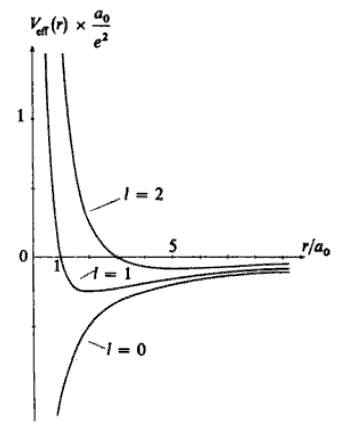
\includegraphics[width=0.33\textwidth]{h-atom_pics/Veff.png}
	\caption{H-Atom Effektives Potential. Form des effektiven Potentials \(V_{eff}(r)\) für die ersten Werte von l für ein Coulomb-Potential \(V(r) = -\frac{e^2}{r}\). Für \(l=0\) entspricht \(V_{eff}(r)\) einfach dem Coulomb-Potential. Für \(l=1,2,ect.\) erhält man \(V_{eff}(r)\),indem man das Zentrifugalpotential \(\frac{l(l+1)\hbar^2}{2\mu r^2}\), das für \(r\to 0\) wie \(\frac{1}{r^2}\) gegen \(+\infty\) läuft, zu \(V(r)\) addiert. Quelle: Cohen-Tannoudji Band 2 }
	\label{fig:1}
\end{figure}

Als weitere Vereinfachung der Gleichung \eqref{eq:18} können wir sie von links mit \(r\) durchmultiplizieren:

\begin{equation}
  \label{eq:19}
   - \frac{\hbar^2}{2\mu}\frac{d^2}{dr^2}\underbrace{r R(r)}_{u(r)} + \left[\frac{l(l+1)\hbar^2}{2\mu r^2}  - \frac{e^2}{r}\right] \underbrace{r R(r)}_{u(r)}   = E_r \underbrace{r R(r)}_{u(r)}
\end{equation}

Nun können wir einen neuen Ansatz Einführen:

\begin{align}
  \label{eq:30}
  u(r) = rR(r)
\end{align}


\begin{equation}
  \label{eq:20}
    \left[-\frac{\hbar^2}{2\mu}\frac{d^2}{dr^2} + \underbrace{\frac{l(l+1)\hbar^2}{2\mu r^2}}_{\text{Zentrifugalpotential}}  - \frac{e^2}{r}\right] u(r)   = E_r u(r)
\end{equation}

Die Lösung \(u(r)\) muss folgende Randbedinungen erfüllen:

\begin{itemize}
\item \(u(r \to 0)=0  \) Für sehr kleine r sollte die Lösung verschwinden und nicht divergierten, da sonst der Hamilton-Operator \(\to\infty\) divergiert.
\item  \(u(r \to \infty)=0  \) da das Coulombpotential im Unendlichen verschwindet.
\end{itemize}

Zu Verdeutlichung eine kleine Umformung:

\begin{equation}
  \label{eq:22}
   \left[-\frac{\hbar^2}{2\mu}\frac{d^2}{dr^2} + \underbrace{\frac{l(l+1)\hbar^2}{2\mu r^2}}_{\text{stark gegen }\infty}  \overbrace{- \frac{e^2}{r} - E_r}^{\text{weniger stark gegen }\infty}   \right] u(r)   = 0 
\end{equation}

Für \(r\to 0\) dominiert das Zentrifugalpotentail, deshalb können wir schreiben:

\begin{equation}
  \label{eq:21}
  r\to 0: \quad\left[-\frac{\hbar^2}{2\mu}\frac{d^2}{dr^2}+ \frac{l(l+1)\hbar^2}{2\mu r^2}\right] u(r) = 0
\end{equation}

Dies ist eine Eulerische DGL 2-er Ordnung. Der Lösungsansatz für diese Art der DGL ist:

\begin{equation}
  \label{eq:23}
  u(r) = Ar^{l+1}+Br^{-l}
\end{equation}

Da \(u(r)\) an der Stelle \(r=0\) verschwinden muss, muss die Konstante \(B=0\) sein. Somit reduziert sich der Ansatz auf:

\begin{equation}
  \label{eq:24}
  u(r) = Ar^{l+1}
\end{equation}

Betrachte nun die Randbedinung \(u(r\to \infty) = 0\).

\begin{equation}
  \label{eq:25}
  \left[-\frac{\hbar^2}{2\mu}\frac{d^2}{dr^2} + \underbrace{\frac{l(l+1)\hbar^2}{2\mu r^2}}_{\to 0}  \underbrace{- \frac{e^2}{r} }_{\to 0} - E_r  \right] u(r)   = 0 
\end{equation}

Somit ergibt sich folgende DGL:

\begin{equation}
  \label{eq:26}
  r\to \infty: \quad\left[\frac{d^2}{dr^2} - \kappa^2\right]u(r) = 0 \qquad \text{mit }\kappa = \sqrt{\underbrace{\frac{2\mu}{\hbar^2}(-E)}_{>0}}
\end{equation}

Mit der Lösung:

\begin{equation}
  \label{eq:27}
  u(r) = Ce^{\kappa r}+De^{-\kappa r}
\end{equation}

Durch die Randbedingung muss \(C=0\) sein somit:

\begin{equation}
  \label{eq:28}
    u(r) = De^{-\kappa r}
\end{equation}

Die Gesamtlösung für \(u(r)\) kann kombiniert werden aus \eqref{eq:24} und \eqref{eq:28}:

\begin{equation}
  \label{eq:29}
  u(r) = r^{l+1}f(r)e^{-\kappa r}
\end{equation}

Wobei \(f(r)\) eine noch zu bestimmende Funktion ist.  

Wir setzen \(u(r)\) in \eqref{eq:22} ein:

\begin{align*}
  \left[-\frac{\hbar^2}{2\mu}\frac{d^2}{dr^2} + \frac{l(l+1)\hbar^2}{2\mu r^2}- \frac{e^2}{r} + \frac{\hbar^2 \kappa^2}{2\mu}  \right] r^{l+1}f(r)e^{-\kappa r}   &= 0 \\
\left[\frac{d^2}{dr^2} + \frac{l(l+1)}{r^2}- \frac{2\mu}{\hbar^2}\frac{e^2}{r} + \kappa^2  \right] r^{l+1}f(r)e^{-\kappa r}   &= 0 \\ 
\frac{d}{dr}\left\{f(r)e^{-\kappa r} \frac{d}{dr}r^{l+1}+ r^{l+1}e^{-\kappa r}\frac{d}{dr} f(r) + r^{l+1} f(r)\frac{d}{dr}e^{-\kappa r}\right\}\\ - \left[\frac{l(l+1)}{r^2}- \frac{2\mu}{\hbar^2}\frac{e^2}{r} + \kappa^2  \right] r^{l+1} f(r)e^{-\kappa r}   &= 0 \\ 
\frac{d}{dr}\left\{f(r)e^{-\kappa r}(l+1)r^{l}+ r^{l+1}e^{-\kappa r}\frac{d}{dr} f(r) - r^{l+1} f(r)\kappa e^{-\kappa r}\right\} \\- \left[\frac{l(l+1)}{r^2}- \frac{2\mu}{\hbar^2}\frac{e^2}{r} + \kappa^2  \right] r^{l+1} f(r)e^{-\kappa r}   &= 0 \\
\left\{ e^{-\kappa r}(l+1)r^{l} \frac{d}{dr}f(r) +  f(r)\frac{d}{dr} e^{-\kappa r}(l+1)r^{l}+f(r)  e^{-\kappa r}(l+1)\frac{d}{dr}r^{l} +\right.\qquad&\\
+e^{-\kappa r}\frac{d}{dr} f(r)\frac{d}{dr}r^{l+1} +r^{l+1}\frac{d}{dr} f(r)\frac{d}{dr}e^{-\kappa r}+r^{l+1}e^{-\kappa r}\frac{d^2}{dr^2} f(r)+\qquad&\\
\left.- f(r)\kappa e^{-\kappa r}\frac{d}{dr}r^{l+1}-r^{l+1}\kappa e^{-\kappa r} \frac{d}{dr}f(r)-r^{l+1} f(r)\kappa \frac{d}{dr}e^{-\kappa r}\right\} \qquad&\\
- \left[\frac{l(l+1)}{r^2}- \frac{2\mu}{\hbar^2}\frac{e^2}{r} + \kappa^2  \right] r^{l+1} f(r)e^{-\kappa r}   &= 0 \\
\left\{ e^{-\kappa r}(l+1)r^{l} \frac{d}{dr}f(r) - \kappa f(r) e^{-\kappa r}(l+1)r^{l}+f(r)  e^{-\kappa r}(l+1)lr^{l-1} +\right.\qquad&\\
+e^{-\kappa r}\frac{d}{dr} f(r)(l+1)r^{l} -\kappa r^{l+1}\frac{d}{dr} f(r)e^{-\kappa r}+r^{l+1}e^{-\kappa r}\frac{d^2}{dr^2} f(r)+\qquad&\\
\left.- f(r)\kappa e^{-\kappa r}(l+1)r^{l}-r^{l+1}\kappa e^{-\kappa r} \frac{d}{dr}f(r)+r^{l+1} f(r)\kappa^2 e^{-\kappa r}\right\} \qquad&\\
- \left[\frac{l(l+1)}{r^2}- \frac{2\mu}{\hbar^2}\frac{e^2}{r} + \kappa^2  \right] r^{l+1} f(r)e^{-\kappa r}   &= 0 |:r^{l+1}:e^{-\kappa r}\\
\left\{(l+1)r^{-1} \frac{d}{dr}f(r) - \kappa f(r) (l+1)r^{-1}+f(r)  (l+1)lr^{-2} +\right.\qquad&\\
+\frac{d}{dr} f(r)(l+1)r^{-1} -\kappa \frac{d}{dr} f(r)+\frac{d^2}{dr^2} f(r)+\qquad&\\
\left.- f(r)\kappa (l+1)r^{-1}-\kappa \frac{d}{dr}f(r)+ f(r)\kappa^2  \right\}\qquad&\\
- \left[\frac{l(l+1)}{r^2}- \frac{2\mu}{\hbar^2}\frac{e^2}{r} + \kappa^2  \right]f(r)   &= 0\\
\left\{2(l+1)r^{-1} \frac{d}{dr}f(r) - 2\kappa f(r) (l+1)r^{-1}+f(r)  (l+1)lr^{-2} -2\kappa \frac{d}{dr} f(r)+\right.\qquad& \\ 
\left. + \frac{d^2}{dr^2} f(r) +  f(r)\kappa^2  \right\}\qquad&\\
- \left[\frac{l(l+1)}{r^2}- \frac{2\mu}{\hbar^2}\frac{e^2}{r} + \kappa^2  \right]f(r)   &= 0\\
\left\{\frac{d^2}{dr^2} + 2\left((l+1)r^{-1}-\kappa\right)\frac{d}{dr} - 2\kappa (l+1)r^{-1}+\cancel{(l+1)lr^{-2}} +  \cancel{\kappa^2}  \right\} f(r) \qquad&\\
- \left[\cancel{ \frac{l(l+1)}{r^2}} - \frac{2\mu}{\hbar^2}\frac{e^2}{r} + \cancel{\kappa^2}  \right]f(r)   &= 0\\
\left\{\frac{d^2}{dr^2} + 2\left((l+1)r^{-1}-\kappa\right)\frac{d}{dr} - 2\kappa (l+1)r^{-1}+ \frac{2\mu}{\hbar^2}\frac{e^2}{r} \right\}f(r)   &= 0
\end{align*}

und erhalten schlussendlich:

\begin{align}
  \label{eq:31}
  \left[ \frac{d^2}{dr^2} + 2\left(\frac{l+1}{r}-\kappa\right)\frac{d}{dr} + 2 \left(-\kappa (l+1) + \frac{\mu e^2}{\hbar^2}\right) \frac{1}{r}  \right] f(r)&= 0
\end{align}

Für \(f(r)\) versuchen wir ein Potenzreihen-Ansatz:

\begin{align}
  \label{eq:32}
  f(r) = \sum^{\infty}_{k=0} b_k r^k
\end{align}
Einsetzen in Gleichung \eqref{eq:31}:

\begin{align*}
 \sum^{\infty}_{k=0} \left[ k(k-1) b_k r^{k-2} + 2\left(\frac{l+1}{r}-\kappa\right)b_k k r^{k-1} + 2 \left(-\kappa (l+1) + \frac{\mu e^2}{\hbar^2}  \right) \frac{1}{r}  b_k r^k \right]  &= 0 \\
 \sum^{\infty}_{k=0} \left[ k(k-1) b_k r^{k-2} + 2(l+1)b_k k r^{k-2}-2\kappa b_k k r^{k-1} + 2 \left(-\kappa (l+1) + \frac{\mu e^2}{\hbar^2}  \right)   b_k r^{k-1} \right]  &= 0 \\
 \sum^{\infty}_{k=0} \left[ (k+2l+1)b_k k r^{k-2}+ 2 \left(-k\kappa-\kappa (l+1) + \frac{\mu e^2}{\hbar^2}  \right)   b_k r^{k-1} \right]  &= 0
\end{align*}

Somit erhalten wir:

\begin{align}
  \label{eq:34}
   \sum^{\infty}_{k=0} \left[ (k+2l+1)b_k k r^{k-2}+ 2 \left(-\kappa(k+l+1) + \frac{\mu e^2}{\hbar^2}  \right)   b_k r^{k-1} \right]  &= 0 
\end{align}

Aus der Gleichung \eqref{eq:34} ergibt sich folgende Rekursionsformel, indem man im letzten Term \(k\) durch \(k-1\) ersetzt:

\begin{align}
  \label{eq:35}
  k(k+2l+1)b_k = 2\left[ \kappa(k+l)-\frac{\mu e^2}{\hbar^2}\right] b_{k-1}
\end{align}

Nun betrachten wir den Quotient von \(b_k\) und Limes:

\begin{align}
  \frac{b_k}{b_{k-1}} &= \frac{2[\kappa(k+l)-\frac{\mu e^2}{\hbar^2}]}{ k(k+2l+1)} 
 = \frac{2k[\kappa(1+\frac{1}{k})-\frac{\mu e^2}{\hbar^2 k}]}{ k(k+2l+1)} 
 = \frac{2[\kappa(1+\frac{1}{k})-\frac{\mu e^2}{\hbar^2 k}]}{ (k+2l+1)}
 = \frac{2\kappa+\frac{2\kappa}{k}-\frac{2\mu e^2}{\hbar^2 k}}{ k(1+\frac{2l}{k}+\frac{1}{k})}\notag\\
 &\xrightarrow{k\to \infty}  \frac{2\kappa+\cancel{\frac{2\kappa}{k}}-\cancel{\frac{2\mu e^2}{\hbar^2 k}}}{ k(1+\cancel{\frac{2l}{k}}+\cancel{\frac{1}{k})}}\notag\\
&\xrightarrow{k\to \infty}  \frac{2\kappa}{k}\label{eq:36}
\end{align}

Gleichung \eqref{eq:36} können wir mit Ausnutzung der Rekursion schreiben:

\begin{align}
  \label{eq:37}
  b_k &= \frac{2\kappa}{k}\cdot b_{k-1} = \frac{2\kappa}{k}\cdot \frac{2\kappa}{k-1} b_{k-2} = \frac{2\kappa}{k}\cdot \frac{2\kappa}{k-1} \frac{2\kappa}{k-2}\cdots \frac{2\kappa}{3}  \frac{2\kappa}{2}  \frac{2\kappa}{1} \cdot b_0 \\
b_k &=  \frac{2^k\kappa^k}{k!}\cdot b_0
\end{align}

Eingesetzt in unseren Potenzreihen-Ansatz \eqref{eq:32}

\begin{align}
  \label{eq:38}
    f(r) = \sum^{\infty}_{k=0} \frac{2\kappa^k}{k!}\cdot b_0  r^k = b_0 \sum^{\infty}_{k=0} \frac{(2\kappa r)^k}{k!} = b_0 e^{2\kappa r} 
\end{align}

Unser Ansatz \eqref{eq:29} lautet nun:

\begin{align}
  \label{eq:39}
    u(r) = b_0 r^{l+1} e^{\kappa r}
\end{align}

Für \(r\to\infty\) wird \(u(r)\) ebenfalls unendlich, was der zweiten Randbedinung widerspricht! 


\subsection{Quantisierung der Energie}

Das Problem, das für \(r\to\infty\) \(u(r)\to\infty\)  kann vermieden werden, wenn wir die Potentzreihe bei einem festen \(N\) abbricht bzw. alle Therme \(>N\) verschwinden. Damit lautet unsere neue Potenz-Reihen Ansatz:

\begin{align}
  \label{eq:40}
 f(r) = \sum^{N}_{k=0} b_kr^k
\end{align}

Betrachten wir nun erneut unsere Rekursionsformel \eqref{eq:35} mit \(k\to k+1\):

\begin{align}
  \label{eq:41}
      k(k+2l+1)b_{k+1} = 2\left[ \kappa(k+l+1)-\frac{\mu e^2}{\hbar^2}\right] b_{k}
\end{align}

und setzen die maximal Zahl \(N\) ein, welche das Verschwinden der \(b_{N+1}\) Terme fordert:

\begin{align}
  \label{eq:42}
    N(N+2l+1)\underbrace{b_{N+1}}_{\stackrel{!}=0} = 2\left[ \kappa(N+l+1)-\frac{\mu e^2}{\hbar^2}\right] b_{N} 
\end{align}

\begin{align}
  \Rightarrow 0 = 2\left[ \kappa(N+l+1)-\frac{\mu e^2}{\hbar^2}\right] b_{N} \\
\Leftrightarrow  \kappa \underbrace{(N+l+1)}_{\equiv n} = \frac{\mu e^2}{\hbar^2}\\
\Leftrightarrow  \kappa= \frac{\mu e^2}{\hbar^2 n}\label{eq:43}
\end{align}
Einsetzen in \eqref{eq:26}

\begin{align}
  \label{eq:44}
  \frac{\mu e^2}{\hbar^2 n} = \sqrt{\frac{2\mu}{\hbar^2}(-E)} \\
\Leftrightarrow  E =  - \frac{\mu e^4}{2\hbar^2 n^2} 
\end{align}

Wir erhalten also die Energienivous für das Wasserstoffatom mit dem Bohr-Radius \(a_0 = \frac{\hbar^2}{\mu e^2}\):

\begin{align}
  \label{eq:46}
  \boxed{E_n =  - \frac{\mu e^4}{2\hbar^2 n^2} = -  \frac{e^2}{2a_0}\frac{1}{n^2} }
\end{align}

Klein \(n\) ist unsere Haupt-Energie-Quantenzahl, und groß \(N\) ist die Radial-Quanten-Zahl und \(l\) ist Drehimpuls-Qaunten-Zahl.

\begin{align}
  \label{eq:45}
  n = N+l+1
\end{align}

Zu bemerken ist, da \(N=0,1,2,3,\cdots\) die erlaubten Werte von \(n\) sind positive ganzen Zahlen \(n=l+1,l+2,l+3,l+4\cdots\). Daraus folgt, dass für ein gegeben Wert für \(n\), die Orbital-Quanten-Zahl \(l\) kann folgende Werte annehmen \(l=n-1,n-2,n-3,n-4,\dots,2,1,0\).


\subsection{Radiale Wellenfunktion}

Nun können wir mit Hilfe der Gleichungen \eqref{eq:30},\eqref{eq:29},\eqref{eq:40} ... die radiale Wellenfunktion zusammensetzen:

\begin{align}
  \label{eq:33}
  R(r) &= \frac{1}{r} r^{l+1}e^{-\kappa r}\sum^{N}_{k=0} b_kr^k \\
&= r^{l}e^{-\kappa r}\sum^{N}_{k=0} b_kr^k \\
\end{align}
Um die radiale Wellenfunktion normieren zu können, führen wir noch eine Normierungskonstante \(A_{nl}\). Damit sieht unsere radiale Wellenfunktion wie folgt aus:

\begin{align}
  \label{eq:47}
   R_{n,l}(r) = A_{nl}r^{l}e^{-\kappa r}\sum^{N}_{k=0} b_kr^k
\end{align}

Mit \(\kappa = \frac{1}{a_0 n}\) lautet die Gleichung \eqref{eq:47} wie folgt:

\begin{align}
  \label{eq:48}
   \boxed{R_{n,l}(r) = A_{nl}r^{l}e^{-\frac{r}{a_0 n}}\sum^{N}_{k=0} b_kr^k}
\end{align}

Mit der Gleichung \eqref{eq:48} können wir nun die radiale Wellenfuktion bestimmen, indem wir für \(n,l\) bestimmte Quantenzahlen einsetzen. Z.B. \(n=1\) und \(l=0\). Und mit Hilfe der Gleichung \eqref{eq:45} folgt für \(N=0\). Eingesetzt in \eqref{eq:48}:

\begin{align}
  \label{eq:49}
  R_{1,0}(r) &= A_{10}r^{0}e^{-\frac{r}{a_0 \cdot 1}}\sum^{0}_{k=0} b_kr^k\\
&= A_{10}e^{-\frac{r}{a_0 }}b_0\\
\end{align}
Die Konstanten werden durch die Normierungsbedinung bestimmt:

\begin{align}
  \label{eq:50}
  1 &= \int_{-\infty}^{\infty} |R_{1,0}(r)|^2d^3r = \int_{0}^{\infty} r^2 |R_{1,0}(r)|^2 dr\\
&=  |A_{10}b_0|^2 \int_{0}^{\infty} r^2e^{-2\frac{r}{a_0 }}\\
&=  |A_{10}b_0|^2  \frac{a_0^3}{4}
\end{align}

Daraus folgt, dass 

\begin{align}
  \label{eq:51}
  A_{10}b_0 = \sqrt{ \frac{4}{a_0^3}} = \frac{2}{\sqrt{a_0^3}}
\end{align}

Die radial Funktion lautet dann:

\begin{align}
  \label{eq:52}
  R_{1,0}(r)= \frac{2}{\sqrt{a_0^3}} e^{-\frac{r}{a_0 }}
\end{align}

So ist es möglich durch einsetzen der Quantenzahlen sukzessive alle radialen Zustände bestimmen.


\subsection*{Laguerre Polynome}

Den Radialanteil kann man auch mittels der zugeordneten Laguerre Polynome ausdrücken. Sie lauten:

\begin{align}
  \label{eq:53}
  L_k^N (r) = \frac{d^N}{dr^N}L_k(r) \qquad \text{mit  } L_k(r) = e^r\frac{d^k}{dr^k}(r^k e^{-r})
\end{align}

Sie lösen folgende Differentialgleichung:

\begin{align}
  \label{eq:54}
  r\frac{d^2}{dr^2}L^N_k(r) + (N+1-r)\frac{d}{dr}L^N_k(r) + (k-N)L^N_k(r) = 0
\end{align}

D.h. wir müssen die Gleichung \eqref{eq:31} in die Form \eqref{eq:54} bringen.

\begin{align}
  \left[ \frac{d^2}{dr^2} + 2\left(\frac{l+1}{r}-\kappa\right)\frac{d}{dr} + 2 \left(-\kappa (l+1) + \frac{\mu e^2}{\hbar^2}\right) \frac{1}{r}  \right] f(r)&= 0 \qquad | \cdot \frac{r}{2\kappa} \\
\left[  \frac{r}{2\kappa} \frac{d^2}{dr^2} + ((2l+1)+1-2\kappa r)\frac{1}{2\kappa}\frac{d}{dr} + (-l-1+\frac{\mu e^2}{\hbar^2 \kappa})  \right] f(r)&= 0 \qquad \text{mit \eqref{eq:43} } n = \frac{\mu e^2}{\hbar^2 \kappa} \\
\left[ \frac{r}{2\kappa} \frac{d^2}{dr^2} + ((2l+1)+1-2\kappa r)\frac{1}{2\kappa}\frac{d}{dr} + (n-l-1)  \right] f(r)&= 0 \\
\left[ \frac{r}{2\kappa} \frac{d^2}{dr^2} + ((2l+1)+1-2\kappa r)\frac{1}{2\kappa}\frac{d}{dr} + (n-l-1+l-l)  \right] f(r)&= 0 \\
\left[ \frac{r}{2\kappa} \frac{d^2}{dr^2} + ((2l+1)+1-2\kappa r)\frac{1}{2\kappa}\frac{d}{dr} + [(n+l)-(2l+1)]  \right] f(r)&= 0 \\
 \label{eq:55}
\end{align}

Substituiere \(r\) durch eine dimensionslose Variablen \(\rho = 2\kappa r\). Daraus ergeben sich auch Substitutionen für die erste und zweite Ableitung:

\begin{align}
  \label{eq:56}
  \rho = 2\kappa r \qquad \Leftrightarrow \qquad r = \frac{\rho}{2\kappa} 
\end{align}

\begin{align}
  \label{eq:57}
  \frac{d}{dr} &= \frac{d}{dr}\frac{d\rho}{d\rho} = \frac{d\rho}{dr}\frac{d}{d\rho} = 2\kappa \frac{d}{d\rho} \\
  \frac{d^2}{dr^2} &= \frac{d}{dr}\frac{d\rho}{d\rho} \frac{d}{dr}\frac{d\rho}{d\rho}= \frac{d\rho}{dr}\frac{d}{d\rho}\frac{d\rho}{dr}\frac{d}{d\rho} = (2\kappa)^2 \frac{d^2}{d\rho^2}
\end{align}

Setze nun die Substitutionen \eqref{eq:56} und \eqref{eq:57} in \eqref{eq:55} ein:

\begin{align}
  \label{eq:58}
  \left[ \frac{\rho}{\cancel{(2\kappa)^2}}\cancel{(2\kappa)^2} \frac{d^2}{d\rho^2}   + ((2l+1)+1-\rho)\frac{1}{\cancel{2\kappa}}\cancel{2\kappa} \frac{d}{d\rho}  + [(n+l)-(2l+1)]  \right] f(r)&= 0\\
  \left[ \rho \frac{d^2}{d\rho^2}   + (\underbrace{(2l+1)}_{\equiv N}+1-\rho)\frac{d}{d\rho}  + [\underbrace{(n+l)}_{\equiv k}-\underbrace{(2l+1)}_{\equiv N}]  \right] f(r)&= 0
\end{align}

Vergleiche mit der Laguerre DGL \eqref{eq:54} ist die Lösung der \eqref{eq:58} folgender Laguerre Polynom:

\begin{align}
  \label{eq:59}
  L^{2l+1}_{n+l}\left(\rho\right) = L^{2l+1}_{n+l}\left(2\kappa r \right)
\end{align}

Damit können wir die Radialgleichung \eqref{eq:48} in Laguerre Polynomen ausdrücken:


\begin{align}
  \label{eq:60}
  R_{n,l}(r) = A_{nl}r^{l}e^{-\frac{r}{a_0 n}} L^{2l+1}_{n+l}\left(2\kappa r \right)
\end{align}

bzw.

\begin{align}
  \label{eq:61}
   R_{n,l}(r) = N_{nl}\left(\frac{2r}{n a_0}\right)^{l}e^{-\frac{r}{a_0 n}} L^{2l+1}_{n+l}\left(\frac{2r}{n a_0}\right)
\end{align}

Aus der Normalisierungsbedingung 

\begin{align}
  \label{eq:62}
  \int^\infty_0 r^2 R^2_{nl} (r) dr = 1
\end{align}

ergibt sich :

\begin{align}
  \label{eq:63}
  N_{nl} = -\left(\frac{2}{na_0}\right)^{\frac{3}{2}}\sqrt{\frac{(n-l-1)!}{2n[(n+1)!]^3} }
\end{align}

Die Konstante \eqref{eq:63} eingesetzt in \eqref{eq:61} erhalten wir die Radialwellenfunktion:

\begin{align}
  \label{eq:64}
 \boxed{ R_{n,l}(r) = -\left(\frac{2}{na_0}\right)^{\frac{3}{2}}\sqrt{\frac{(n-l-1)!}{2n[(n+1)!]^3} } \left(\frac{2r}{n a_0}\right)^{l}e^{-\frac{r}{a_0 n}} L^{2l+1}_{n+l}\left(\frac{2r}{n a_0}\right)}
\end{align}

Die Gesamtwellenfunktion \eqref{eq:17} lautet schlussendlich:


\begin{align}
  \label{eq:65}
  \psi_{nlm}(r,\theta,\phi) = R_{nl}(r)\cdot Y_{lm}(\theta,\phi)
\end{align}








\end{document}
